% Preamble: \usepackage{booktabs,tabularx,graphicx,tikz}
%           \usetikzlibrary{positioning,arrows.meta,calc}
\section{Methodology}
\label{sec:method}

We start from the 731 tasks of the original SWE-Bench Pro Public. A task consists of an instruction (problem statement, requirements, new interfaces), a container image with the repository at its base commit, a reference patch, a hidden test patch, fail-to-pass and pass-to-pass lists naming the graded tests, and a verifier that applies the test patch, runs the tests and parses the output. A task is valid if every solution that satisfies the instruction passes and every solution that does not, fails. Our agentic audits flagged 200 tasks (27\%), and engineers adjudicated each flag (Figure~\ref{fig:pipeline}). The released set has 642 tasks: 531 never flagged, 66 repaired and 45 flagged but kept unchanged. The remaining 89 were discarded.

% Pipeline figure for Section~\ref{sec:method}: flow of the 731 tasks.
% Band and bar heights are proportional to task counts (0.046 mm per task).
% Preamble: \usepackage{tikz,graphicx} (xcolor is loaded by tikz)
\definecolor{sbpFlag}{HTML}{4C72B0}
\definecolor{sbpRep}{HTML}{55A868}
\definecolor{sbpDisc}{HTML}{C44E52}
\definecolor{sbpKeep}{HTML}{7F7F7F}
\definecolor{sbpNone}{HTML}{B0B0B0}
\begin{figure*}[t]
\centering
\resizebox{\textwidth}{!}{%
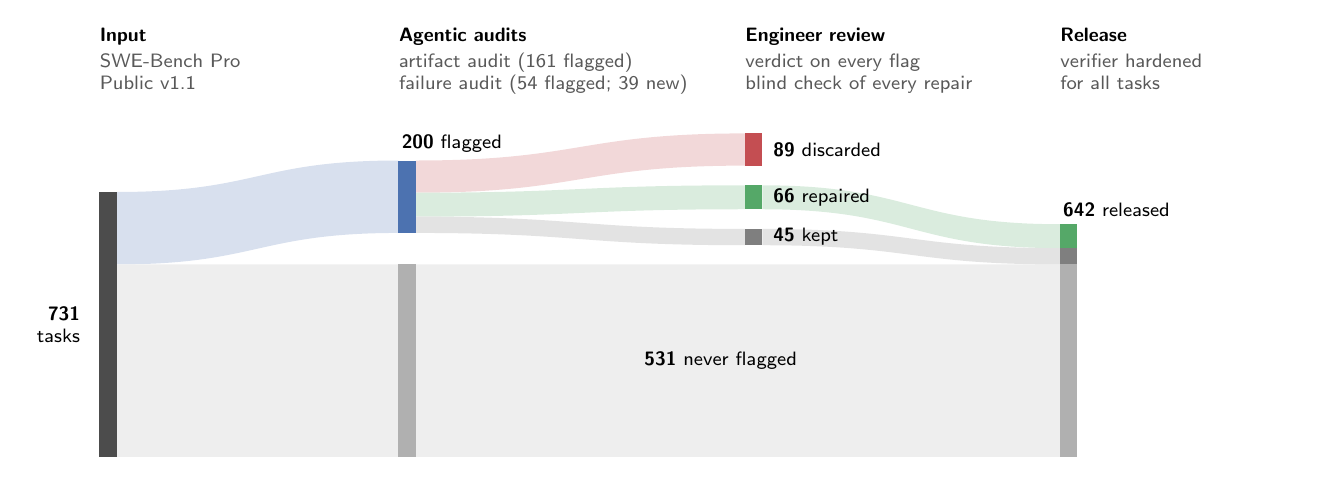
\begin{tikzpicture}[x=1mm, y=1mm, font=\sffamily\scriptsize,
  execute at begin node={\hyphenpenalty=10000\exhyphenpenalty=10000}]
% flagged by an audit
\fill[sbpFlag!22] (2.2,4.09) .. controls (20.1,4.09) and (20.1,8.09) .. (38,8.09)
  -- (38,-1.11) .. controls (20.1,-1.11) and (20.1,-5.11) .. (2.2,-5.11) -- cycle;
% never flagged
\fill[sbpNone!22] (2.2,-5.11) .. controls (20.1,-5.11) and (20.1,-5.11) .. (38,-5.11)
  -- (38,-29.54) .. controls (20.1,-29.54) and (20.1,-29.54) .. (2.2,-29.54) -- cycle;
% discarded
\fill[sbpDisc!22] (40.2,8.09) .. controls (61.1,8.09) and (61.1,11.53) .. (82,11.53)
  -- (82,7.44) .. controls (61.1,7.44) and (61.1,4) .. (40.2,4) -- cycle;
% repaired
\fill[sbpRep!22] (40.2,4) .. controls (61.1,4) and (61.1,4.94) .. (82,4.94)
  -- (82,1.9) .. controls (61.1,1.9) and (61.1,0.96) .. (40.2,0.96) -- cycle;
% kept unchanged
\fill[sbpKeep!22] (40.2,0.96) .. controls (61.1,0.96) and (61.1,-0.6) .. (82,-0.6)
  -- (82,-2.67) .. controls (61.1,-2.67) and (61.1,-1.11) .. (40.2,-1.11) -- cycle;
% never flagged, passes review
\fill[sbpNone!22] (40.2,-5.11) .. controls (81.1,-5.11) and (81.1,-5.11) .. (122,-5.11)
  -- (122,-29.54) .. controls (81.1,-29.54) and (81.1,-29.54) .. (40.2,-29.54) -- cycle;
% repaired -> release
\fill[sbpRep!22] (84.2,4.94) .. controls (103.1,4.94) and (103.1,0) .. (122,0)
  -- (122,-3.04) .. controls (103.1,-3.04) and (103.1,1.9) .. (84.2,1.9) -- cycle;
% kept -> release
\fill[sbpKeep!22] (84.2,-0.6) .. controls (103.1,-0.6) and (103.1,-3.04) .. (122,-3.04)
  -- (122,-5.11) .. controls (103.1,-5.11) and (103.1,-2.67) .. (84.2,-2.67) -- cycle;
% nodes
\fill[black!70] (0,-29.54) rectangle (2.2,4.09);
\fill[sbpFlag] (38,-1.11) rectangle (40.2,8.09);
\fill[sbpNone] (38,-29.54) rectangle (40.2,-5.11);
\fill[sbpDisc] (82,7.44) rectangle (84.2,11.53);
\fill[sbpRep] (82,1.9) rectangle (84.2,4.94);
\fill[sbpKeep] (82,-2.67) rectangle (84.2,-0.6);
\fill[sbpRep] (122,-3.04) rectangle (124.2,0);
\fill[sbpKeep] (122,-5.11) rectangle (124.2,-3.04);
\fill[sbpNone] (122,-29.54) rectangle (124.2,-5.11);
% labels
\node[anchor=east, align=right] at (-1.2,-12.72) {\textbf{731}\\tasks};
\node[anchor=south west, inner sep=1pt] at (38,8.69) {\textbf{200} flagged};
\node[anchor=west] at (68,-17.32) {\textbf{531} never flagged};
\node[anchor=west, inner sep=1pt] at (85.2,9.48) {\textbf{89} discarded};
\node[anchor=west, inner sep=1pt] at (85.2,3.42) {\textbf{66} repaired};
\node[anchor=west, inner sep=1pt] at (85.2,-1.64) {\textbf{45} kept};
\node[anchor=south west, inner sep=1pt] at (122,0.6) {\textbf{642} released};
% stage headers
\node[anchor=north west, inner sep=0pt, text width=34mm, align=left] at (0,25.03)
  {{\bfseries Input}\\[1.5pt]\textcolor{black!65}{SWE-Bench Pro\\Public v1.1}};
\node[anchor=north west, inner sep=0pt, text width=43mm, align=left] at (38,25.03)
  {{\bfseries Agentic audits}\\[1.5pt]\textcolor{black!65}{artifact audit (161 flagged)\\failure audit (54 flagged; 39 new)}};
\node[anchor=north west, inner sep=0pt, text width=38mm, align=left] at (82,25.03)
  {{\bfseries Engineer review}\\[1.5pt]\textcolor{black!65}{verdict on every flag\\blind check of every repair}};
\node[anchor=north west, inner sep=0pt, text width=30mm, align=left] at (122,25.03)
  {{\bfseries Release}\\[1.5pt]\textcolor{black!65}{verifier hardened\\for all tasks}};
\end{tikzpicture}}%
\caption{Flow of the 731 tasks; bar and band heights are proportional to
task counts. The artifact audit (an LLM agent and a human auditor compare the
instruction with the tests and reference patch) and the failure audit (an LLM
judge attributes failed runs of four agent setups) flag 200 tasks. Engineers
adjudicate every flag, and a repair ships only after a blind re-implementation
of the edited instruction passes the hidden tests.}
\label{fig:pipeline}
\end{figure*}


\subsection{Agentic audits}
\label{sec:audits}

\paragraph{Artifact audit.}
An LLM agent compared each task's instruction with its test patch, graded-test lists and reference patch, without executing anything. It flagged six patterns: test requirements missing from the instruction, instruction statements contradicted by the tests, test or solution detail copied into the instruction, changed behaviour that no graded test exercises, fixtures read by the tests but never created, and graded lists naming a whole test file. Requirement sections far above the dataset median length (about 2{,}800 characters) were treated as a leakage signal, as they often transcribed the reference patch. A human auditor reviewed the agent's flags, and marked high-priority cases. The final audit flagged 161 tasks. 

\paragraph{Failure audit.}
We ran four agent configurations on every task: Claude Code with Claude Opus~5, Codex with GPT-5.6, and mini-SWE-agent with each model. For each failed run, an LLM judge read the trajectory, patch, verifier log and graded tests and attributed the failure to the model or to the task. A task was flagged when a patch consistent with a reasonable reading of the instruction was rejected. In one \textit{vuls} task, two configurations fell back to the bundle directory name as instructed and reported \texttt{Sample.app}, while the graded test expects \texttt{Sample} because the reference patch strips the suffix without the instruction saying so. For each flag the judge recorded the defect type, the fix location (instruction, tests, image, graded list or verifier), an effort estimate, a proposed edit, and the passing and failing configurations.
% CHECK: confirm with the audit team that failure attribution was done by an LLM judge.

\subsection{Defect taxonomy}
\label{sec:taxonomy}

We merged the audits' labels into the six categories of Table~\ref{tab:repairs-discards} and assigned each task the defect that determined its outcome. Unstated requirements, contradictions and verifier or environment defects make correct solutions fail. Leakage and insufficient tests make a task easier than intended or let an incomplete solution pass. Table~\ref{tab:problems} maps the categories to data and evaluation problems.

\begin{table}[t]
\centering
\small
\setlength{\tabcolsep}{3pt}
\begin{tabularx}{\columnwidth}{@{}>{\raggedright\arraybackslash}p{2.05cm} >{\raggedright\arraybackslash}X r r@{}}
\toprule
\textbf{Category} & \textbf{Description} & \textbf{Rep.} & \textbf{Disc.} \\
\midrule
Solution leakage & The instruction gives away test or solution detail. & 24 & 4 \\
\addlinespace
Spec--test contradiction & The instruction contradicts what the tests check. & 8 & 5 \\
\addlinespace
Unstated test requirement & The tests require behaviour, names or files the instruction never states. & 31 & 22 \\
\addlinespace
Insufficient tests & The tests miss part of the change or check incidental details instead of behaviour. & 3 & 33 \\
\addlinespace
Verifier or environment defect & The grading setup or container decides the score regardless of the solution. & 0 & 19 \\
\addlinespace
Miscellaneous & -- & -- & 6 \\
\midrule
\textbf{Total} & & \textbf{66} & \textbf{89} \\
\bottomrule
\end{tabularx}
\caption{Defect categories of tasks repaired and kept (Rep.) and discarded (Disc.) between the 731 tasks of SWE-Bench Pro Public v1.1 and the final 642. Repairs edited the instruction in 63 tasks and the test patch in 4 (one task both).}
\label{tab:repairs-discards}
\end{table}

% Needs: \usepackage{booktabs,tabularx}
\begin{table}[t]
\centering\footnotesize
\setlength{\tabcolsep}{3pt}
\begin{tabularx}{\columnwidth}{@{}>{\raggedright\arraybackslash}p{2.05cm}>{\raggedright\arraybackslash}X>{\raggedright\arraybackslash}X@{}}
\toprule
\textbf{Problem} & \textbf{Evidence} & \textbf{Fix} \\
\midrule
\multicolumn{3}{@{}l}{\textit{Data}} \\
Instruction and tests disagree & 94 tasks (Table~\ref{tab:repairs-discards}) & 63 instructions edited; 31 tasks discarded \\
\addlinespace[1.5pt]
Tests too weak & 36 tasks & 3 assertions added; 33 tasks discarded \\
\addlinespace[1.5pt]
Grading or image broken & 19 tasks; shared defects in 253 Go, 322 Python and 47 jest verifiers & 19 tasks discarded; verifiers scoped, capped, re-parsed \\
\addlinespace[1.5pt]
Parser renamed graded tests & Reference patch failed on \nParserFail{} tasks & Graded names regenerated \\
\addlinespace[1.5pt]
Agent files reach grading & 44 runs zeroed; stale bytecode & Test files, test data and bytecode reset before grading \\
\midrule
\multicolumn{3}{@{}l}{\textit{Evaluation}} \\
Open internet & \netTrajOpen{}/\nTasks{} runs reached code hosts; \netOwnRepoOpen{} fetched their own repository & Only the model endpoint reachable; probed before each run \\
\addlinespace[1.5pt]
Web tools outside the sandbox & \webFetchTrajOpen{}/\nTasks{} runs used web fetch & Disabled \\
\addlinespace[1.5pt]
Grading in the agent's sandbox & A \texttt{python3} wrapper scores an empty patch 1 & Re-graded in a clean container \\
\addlinespace[1.5pt]
Fix in git history & \probeImages{} images checked & Fixing commit absent; probed \\
\bottomrule
\end{tabularx}
\caption{Problems found in SWE-Bench Pro and the v2 fix. Data problems concern the tasks; evaluation problems concern how runs are executed and graded.}
\label{tab:problems}
\end{table}

\paragraph{Unstated test requirement (31 repaired, 22 discarded).}
The tests depend on behaviour, names or files the instruction does not mention. In a \textbf{flipt} task, \texttt{TestLoad} reads three YAML samples (\texttt{otlp.yml} with \texttt{samplingRatio} set to 0.5, \texttt{wrong\_sampling\_ratio.yml} and \texttt{wrong\_propagator.yml}) that existed only in the reference patch. The repaired instruction specifies all three. The \textit{vuls} bundle-name task was repaired by stating that the \texttt{.app} suffix is removed. We repaired a task when the missing requirement is behaviour the task is about, and discarded it when the test checks how the reference patch happens to be written, since stating that would give the solution away. Discarded tests read a private attribute (\texttt{\_values} in \textit{qutebrowser}), pin avatar CSS classes in a snapshot (element-web), or inspect a private client through \texttt{reflect} and \texttt{unsafe} (flipt). 

\paragraph{Spec--test contradiction (8 repaired, 5 discarded).}
A vuls instruction said a package is \textit{not affected} when exactly one of the package and the OVAL definition carries a modularity label. Four pre-existing graded cases require the legacy fallback to the host's enabled modules, which the reference patch keeps, and the repair states that fallback. Contradictions whose fix lies in the tests were discarded, for example a \textit{webclients} task whose interface declares an \texttt{Element} argument while the graded test passes a \texttt{Document}.

\paragraph{Solution leakage (24 repaired, 4 discarded).}
Leaky instructions walked through the reference patch file by file, quoted its strings, or copied expected values from the tests. A \textit{tutanota} instruction told the agent to update the try-catch block around \texttt{aes256Decrypt} in \texttt{decrypt}. The repaired version specifies behaviour only: a \texttt{CryptoError} raised by the crypto library must surface as the application's own \texttt{CryptoError}, which the credentials layer converts to \texttt{KeyPermanentlyInvalidatedError}. Repairs delete the leaked text and, where a test depends on it, restate the requirement as behaviour. The four discards were repaired and then removed with a late batch (\S\ref{sec:review}).

\paragraph{Insufficient tests (3 repaired, 33 discarded).}
The graded tests leave part of the change unchecked (28) or assert incidental details (5). In a \textit{flipt} task they cover only the error paths of a new cache layer, so a \texttt{getJSON} that always returns false and a no-op \texttt{setJSON} pass. Engineers did not write tests, so these tasks were discarded. The three repairs are auditor edits that each add one assertion. A \textit{vuls} test now expects an error for an image reference with both a tag and a digest, and a teleport fuzz test now requires the parser error it previously ignored. 

\paragraph{Verifier or environment defect (19 discarded).}
In 16 tasks the fail-to-pass list names a whole file (e.g.\ \texttt{test/tests/calendar/\allowbreak CalendarUtilsTest.js \textbar{} test suite}), so any unrelated or flaky failure in that file fails a correct patch. In 3 tasks the image prevents grading. A vuls test imports a package that exists only in a newer module version than the image's offline Go module cache holds, and a teleport test is skipped because SoftHSM is missing, which the verifier scores as a failure. These tasks needed per-task changes to the graded list or the image, shared verifier defects were fixed globally (\S\ref{sec:verifier}).


\subsection{Engineer review}
\label{sec:review}

Engineers focused on the criteria that if the reference patch adds a behaviour and a hidden test checks it, the instruction must state the behavior, but not how the reference patch implements it. Hidden tests were never edited to agree with an instruction, and instructions were never rewritten to match a wrong test.

23 contracted engineers adjudicated every flag, spending 1{,}897 hours in total. For each claim in a flag they recorded whether it holds, holds in part or does not hold, citing evidence by artifact and line (eg: \texttt{requirements:19}, \texttt{test\_patch\_before:178}, \texttt{f2p:1}, \texttt{golden:562}). A false flag leaves the task unchanged, a flag whose gap is in the instruction leads to an edit limited to where the flag holds, a flag whose remedy lies in the tests, fixtures, verifier or image leads to quarantine, i.e.\ removal. High-priority flags received a second independent review and a third pass by the project team. %The audit team checked all 147 verdicts on its proposed removals and challenged four, which were re-examined.
% CHECK: confirm 23 and 1{,}897 cover the review of all 200 flags, not only the 55 instruction repairs.

For those 147 tasks, reviewers confirmed 70 flags, partly confirmed 21 and rejected 56. The final outcome was 34 repaired, 43 kept and 70 discarded. Of the 54 failure-audit flags, 35 were repaired and 19 discarded. The judge's fix location predicted the outcome well: 28 of the 31 flags it located in the instruction were repaired, and 16 of the 23 located elsewhere were discarded. For the other 7, engineers found a fix, mostly in the instruction (the flipt YAML task is one).

Engineer repairs were validated blind. A second engineer who had seen neither the original task nor the reference patch implemented the edited instruction, and the edit shipped only if that implementation passed the hidden tests. For the auditors' repairs, the reference patch was re-run against the edited tests. Fourteen tasks repaired in a second batch were removed before release, we count them as discards under their original flag, and they include all four leakage discards. Two auditor repairs were not carried into the release, and those tasks are counted as kept. A task counts as repaired only if its instruction or test patch changed in response to a confirmed flag. Release-wide changes are not counted.
% CHECK: add the reason the 14-task batch was removed at release.
% CHECK: the final release also edited instructions of some unflagged tasks and 13 rejected-flag tasks (leak pass); decide whether to disclose these here.

\subsection{Verifier hardening}
\label{sec:verifier}

Defects in shared grading code were fixed for all tasks.

\paragraph{Scoping and resources.}
The Go verifier ran \texttt{go test ./...} over the whole repository. Scoping it to the graded packages on 253 tasks removed out-of-memory failures and timeouts above 150 minutes without changing any grade. Run scripts on 231 tasks that executed the full suite were restricted to the graded tests. With automatic worker counts, pytest-xdist spawned up to 128 workers on small test files and crashed with ``no tests ran'': we capped it at four workers on 239 tasks and inside \texttt{ansible-test} on 83.

\paragraph{Parsing and environment.}
The jest parser assigned tests in failing files to the wrong file and dropped failures (47 tasks), and it truncated test titles at the first parenthesis: it now strips only the trailing timing. We added kernel headers for cgo builds (5 tasks), fetched at grading time one Go module missing from an image's offline cache, re-derived test scoping on 3 tasks that omitted the packages defining the graded tests, and restored CRLF line endings in a fixture that made the reference patch fail.

\paragraph{Test-file reset.}
Before the hidden tests run, the verifier (i)~restores every path the test patch touches and deletes only paths it creates; (ii)~restores modified tracked test data (test data, fixtures, mocks, snapshots), with allowlists for the six reference patches that change fixtures; (iii)~removes agent-written test files that collide with hidden tests; (iv)~clears stale git lock files left by killed agent commands; and (v)~deletes \texttt{\_\_pycache\_\_} and \texttt{.pyc} files. Without (i), agent edits to snapshots owned by the test patch made it fail to apply in 44 runs. Step (v) addresses \texttt{.pyc} files that an agent's \texttt{git stash} round trip left with unchanged size and timestamp, which made the verifier import the base code.

On the assembled 642-task set, the reference patch passes every task and the empty patch fails every task.
% CHECK: re-run the oracle/empty-patch check on the final release package; the 100%/0% result predates the last verifier and instruction updates.

\subsection{Hardened evaluation protocol}
\label{sec:protocol}

We run every model under a locked protocol. The harness sets network access per phase of a run, probes the lock from inside the sandbox before the run starts, and grades the agent's patch in a fresh container rather than in the agent's sandbox. Table~\ref{tab:problems} maps each component to the problem it addresses.

\paragraph{Network.}
With the network open, 32 of 642 Claude Opus~5 trajectories contacted code hosts, and 25 downloaded the task's own repository. Under the lock, the sandbox can reach only the model endpoint during the agent phase; the allowlist names that hostname alone, and the endpoint does not relay other traffic. Web tools that scaffolds execute outside the sandbox are disabled. Before each run, a probe executes in the sandbox under the job's exact flags and aborts the run unless every code host is unreachable, the endpoint answers and the reference patch still passes. The git history of all 642 images contains neither the fixing commit nor any reflog entries, stashes or dangling objects.

\paragraph{Grading.}
The original harness ran the verifier in the sandbox the agent had just used. Because the verifier restores test files but not binaries, a scripted agent that edits no source file and replaces \texttt{python3} with a script printing \textsc{PASSED} scores 1. We saw no model attempt this, but forged dependencies passed through the same gap: with the network closed, some agents that could not fetch a fix edited the Go module cache in place or served a fabricated module version from a local \texttt{GOPROXY}, and neither change appears in the diff. We now save the agent's changes as a patch, apply it to a fresh copy of the task image, run the unchanged verifier there and report that grade. Binaries, module caches, \texttt{node\_modules}, \texttt{site-packages} and \texttt{go env} settings do not carry over.
%We report both grades for every task. When the two disagree, two more fresh grades decide, by majority.
% CHECK: CHEATING_MODES.md says the fresh re-grade is authoritative and that flips are adjudicated with 2 extra fresh re-grades (a forgery fails 2/2, a flake passes at least 1/2). Align the commented sentence with that before re-enabling it.

\paragraph{Audits.}
A fresh re-grade cannot catch a forgery committed inside the patch, so we audit patches for \texttt{replace} directives that point into the patch or to absolute paths, \texttt{go.sum} entries for modules absent from the image, and large new directories that imitate a third-party SDK. We also scan trajectories for fetches that returned content; writes to module caches, package directories or \texttt{/usr/*bin}; and reads of \texttt{/tests} or \texttt{/solution}.
% CHECK: state whether flagged patches are rejected automatically or reviewed by hand.
